\section{USB – Uniwersalny interfejs szeregowy}
	\subsection{Co to jest?}
	\subsection{Parametry}
	Dla USB 1.1 oraz 2.0
	\begin{itemize}
		\item Szybkość transmisji: 12 Mb/s (1.1), 480 Mb/s (2.0)
		\item Złożoność kontrolera w stacji host: 10000 bramek
		\item Złożoność kontrolera w urządzeniu: 1500 do 2000 bramek
	\end{itemize}
	\subsection{Charakterystyka systemu USB}
		\subsubsection{Podstawowe właściwości interfejsu USB}
		\begin{itemize}
			\item \textbf{Gorące podłączenie} - włączanie/wyłączanie urządzeń bez wyłączania systemu.
			\item \textbf{Jeden typ złącza} - złącze typu A w koncentratorze i B w urządzeniu.
			\item \textbf{Duża liczba podłączanych urządzeń} - maksymalnie do 127
			\item \textbf{Różne szybkości transmisji} - mała: 1,5 Mb/s, pełna: 12 Mb/s, wysoka: 480 Mb/s
			\item \textbf{Zasilanie} - system dystrybucji zasilania: 5V/500 mA, zawieszenie, wznowienie, wake-up
			\item \textbf{Protokół komunikacyjny, detekcja błędów} - pakietowy z kontrolą poprawności przesyłu
			\item \textbf{Transfery USB} - 4 typy transferów:
				\begin{itemize}
					\item kontrolny
					\item masowy
					\item przerwaniowy
					\item izochroniczny
				\end{itemize}
			\item \textbf{Niski koszt} - nieduża złożoność układów interfejsowych
			\item \textbf{Schemat blokowy systemu USB}\\
			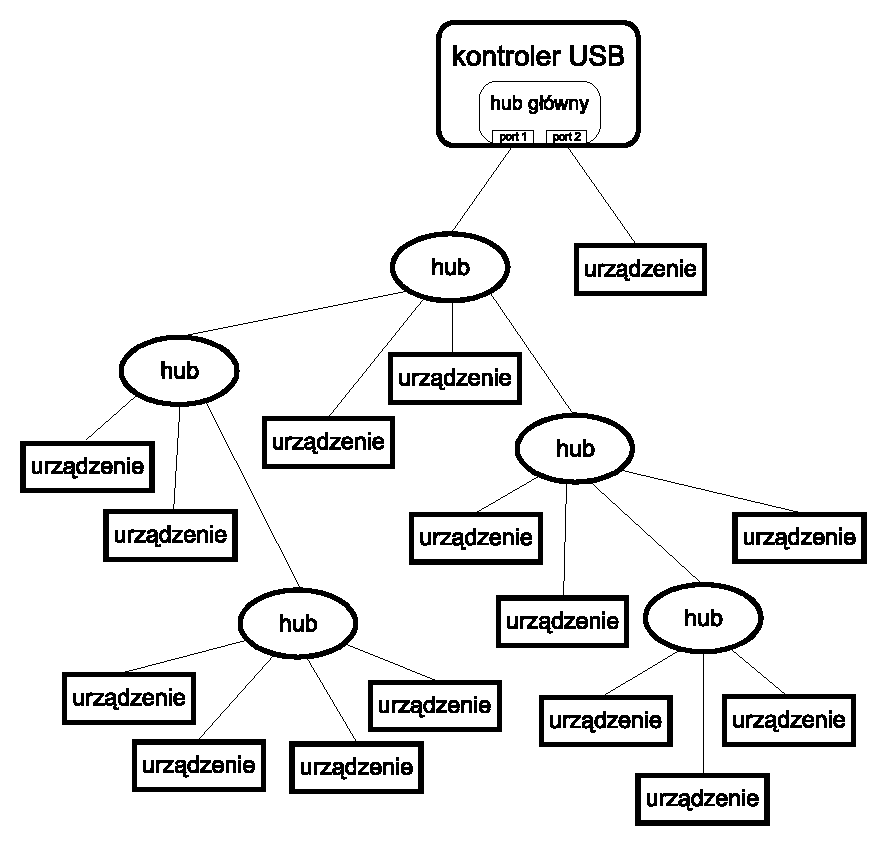
\includegraphics[width=10cm]{./wyklady/USB_6_1.pdf}
		\end{itemize}
		\subsubsection{Środowisko sygnałowe i fizyczne}
			\textbf{Obwód transmisyjny w standardzie USB}\\
			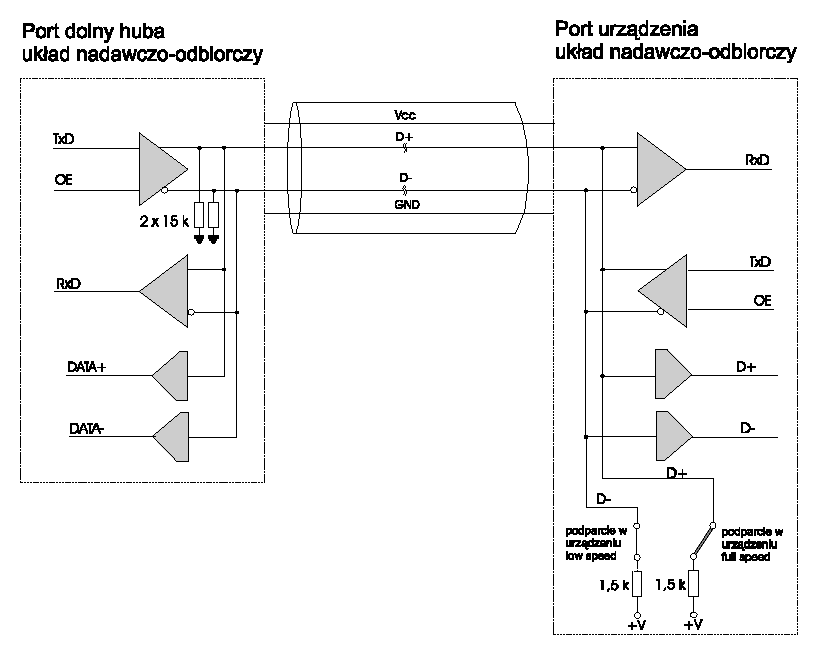
\includegraphics[width=10cm]{./wyklady/USB_7_1.pdf}
			\textbf{Stany magistrali USB}\\
			\begin{itemize}
				\item Logiczne „1” w obwodzie różnicowym (D+) - (D-) $>$ 200 mV
				\item Logiczne „0” w obwodzie różnicowym (D+) - (D-) $<$ -200 mV
				\item Plus 9 innych stanów
			\end{itemize}
			\textbf{Kodowanie NRZI ze wstawianiem bitu synchronizującego}\\
			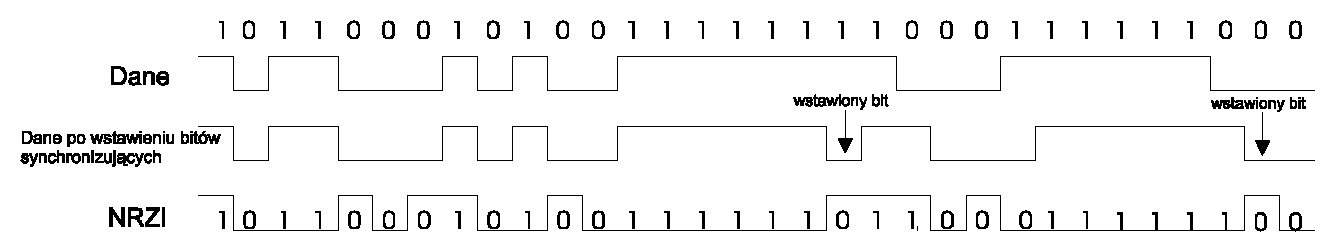
\includegraphics[width=15cm]{./wyklady/USB_9_1.pdf}\\\\
			\textbf{Podstawowy kabel do podłączenia urządzenia USB}\\
			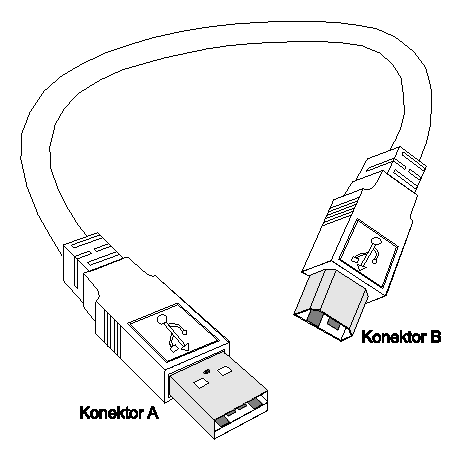
\includegraphics[width=6cm]{./wyklady/USB_10_1.pdf}
			\begin{itemize}
				\item Konektor A – strona portu dolnego (hub)
				\item Konektor B – strona portu górnego (urządzenie)
			\end{itemize}
			\begin{table}[h]
				\begin{tabular}{|c|c|c|}
					\hline
					\textbf{Nr kontaktu}	& \textbf{Nazwa sygnału}	& \textbf{Kolor przewodu w kablu} \\ \hline
					1 						& Vcc						& Czerwony		\\ \hline
					2 						& +DATA						& Biały			\\ \hline
					3 						& -DATA						& Zielony		\\ \hline
					4 						& GND						& Czarny		\\ \hline
				\end{tabular}
			\end{table}
			\textbf{Właściwości}
			\begin{itemize}
				\item Kabel „low speed”
				\begin{itemize}
					\item nieekranowany
					\item dwie, nie skręcane pary przewodów: dla danych (28 AWG) i zasilania (20-28 AWG)
				\end{itemize}
				\item Kabel „full speed i high speed”
				\begin{itemize}
					\item ekranowana para skręcana (28 AWG) dla danych
					\item nieekranowana para (20-28 AWG) dla zasilania
				\end{itemize}
				\item Czas propagacji sygnału w kablu: $<$ 30 ns
			\end{itemize}
		\subsubsection{Ramki i mikro ramki}
			\textbf{Ramki i mikroramki w standardzie USB}\\
			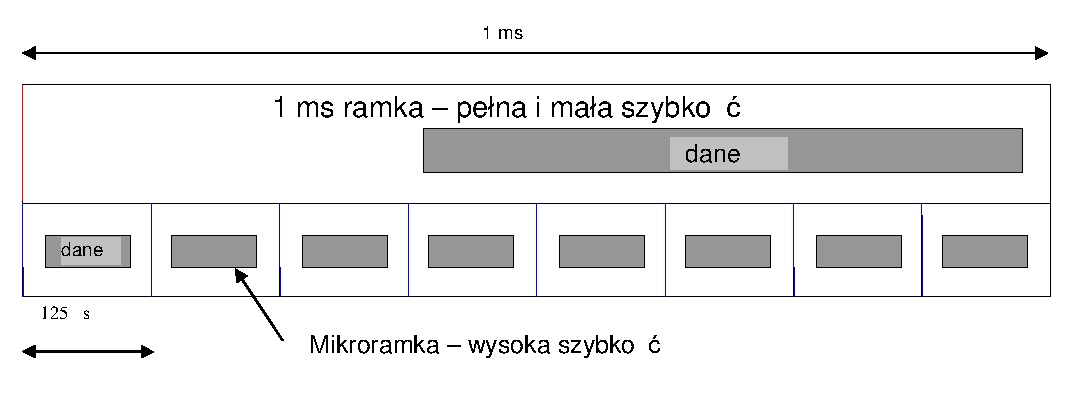
\includegraphics[width=10cm]{./wyklady/USB_11_1.pdf}\\
			\textbf{Właściwości}
			\begin{itemize}
				\item Pełna szybkość transmisji
				\begin{itemize}
					\item Max rozmiar ramki w bitach: 1 ms x 1/12 Mhz = 12000 bitów
					\item Max rozmiar ramki w bajtach: 12000 : 8 = 1500
				\end{itemize}
				\item Mała szybkość transmisji
				\begin{itemize}
					\item Max rozmiar ramki w bitach: 1 ms x 1/1,5 Mhz = 1500 bitów
					\item Max rozmiar ramki w bajtach: 1500 : 8 = 187
				\end{itemize}
				\item Mikroramka 125 $\mu s$
				\begin{itemize}
					\item Mikroramka trwa 125 $\mu s$
					\item Na 1 ramkę przypada 8 mikroramek
				\end{itemize}
				\item Wysoka prędkość transmisji - Szybkość transmisji w mikroramce wynosi 480 Mhz.
			\end{itemize}
		\subsubsection{Model komunikacyjny}
		\textbf{Warstwowy model komunikacyjny}\\
		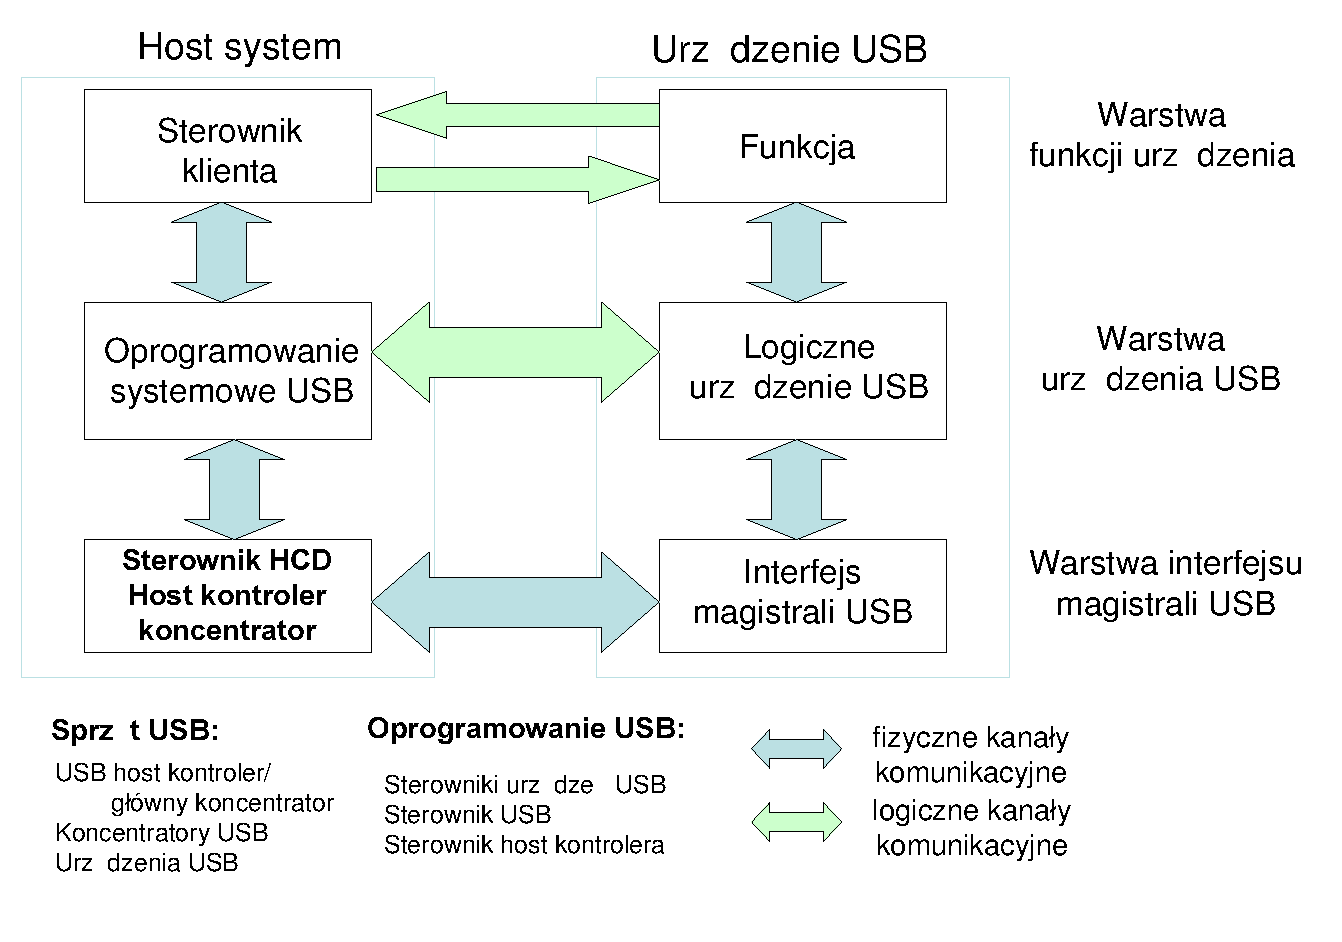
\includegraphics[width=10cm]{./wyklady/USB_12_1.pdf}\\\\
		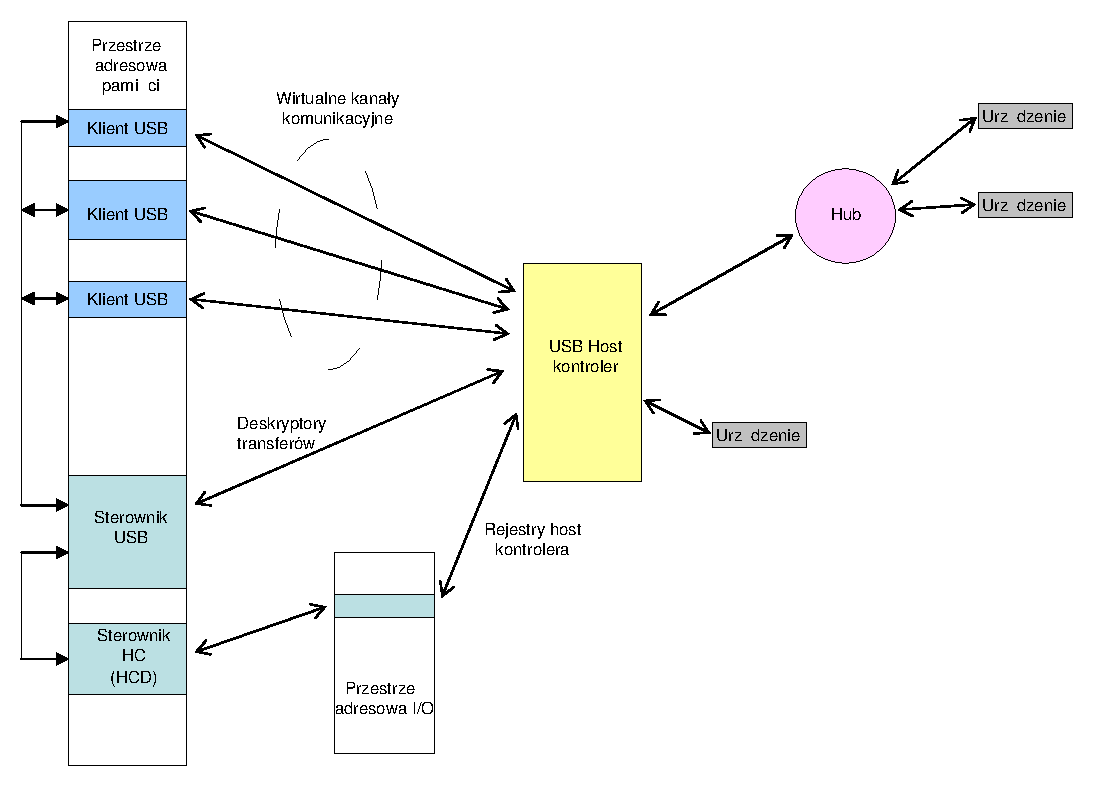
\includegraphics[width=10cm]{./wyklady/USB_13_1.pdf}\\
		\subsubsection{Transfery USB}
		\begin{itemize}
			\item Kontrolny (control transfer) - time delivery accuracy + quality delivery accuracy
			\item Masowy (interrupt transfer) - time delivery accuracy + quality delivery accuracy
			\item Przerwaniowy (bulk transfer) - quality delivery accuracy
			\item Izochroniczny (isochronous transfer) - time delivery accuracy
		\end{itemize}
		\begin{itemize}
			\item Transfery kontrolny i masowy – aperiodyczne
			\item Transfery przerwaniowy i izochroniczny - periodyczne
		\end{itemize}
		\subsubsection{Stany urządzenia USB}
		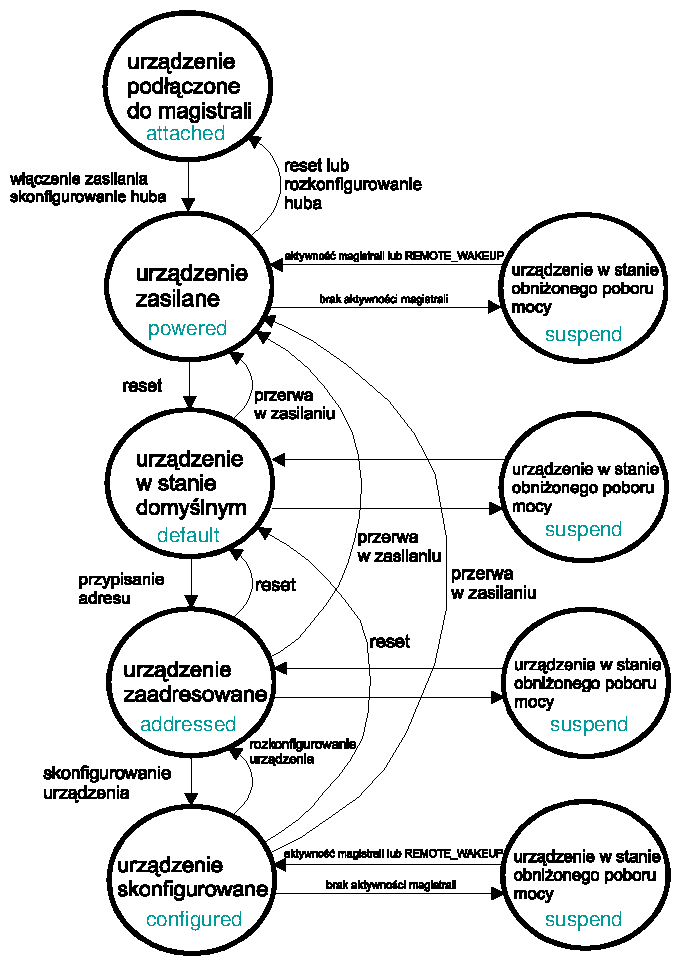
\includegraphics[width=10cm]{./wyklady/USB_16_1.pdf}
		\subsubsection{Hub w systemie USB}
		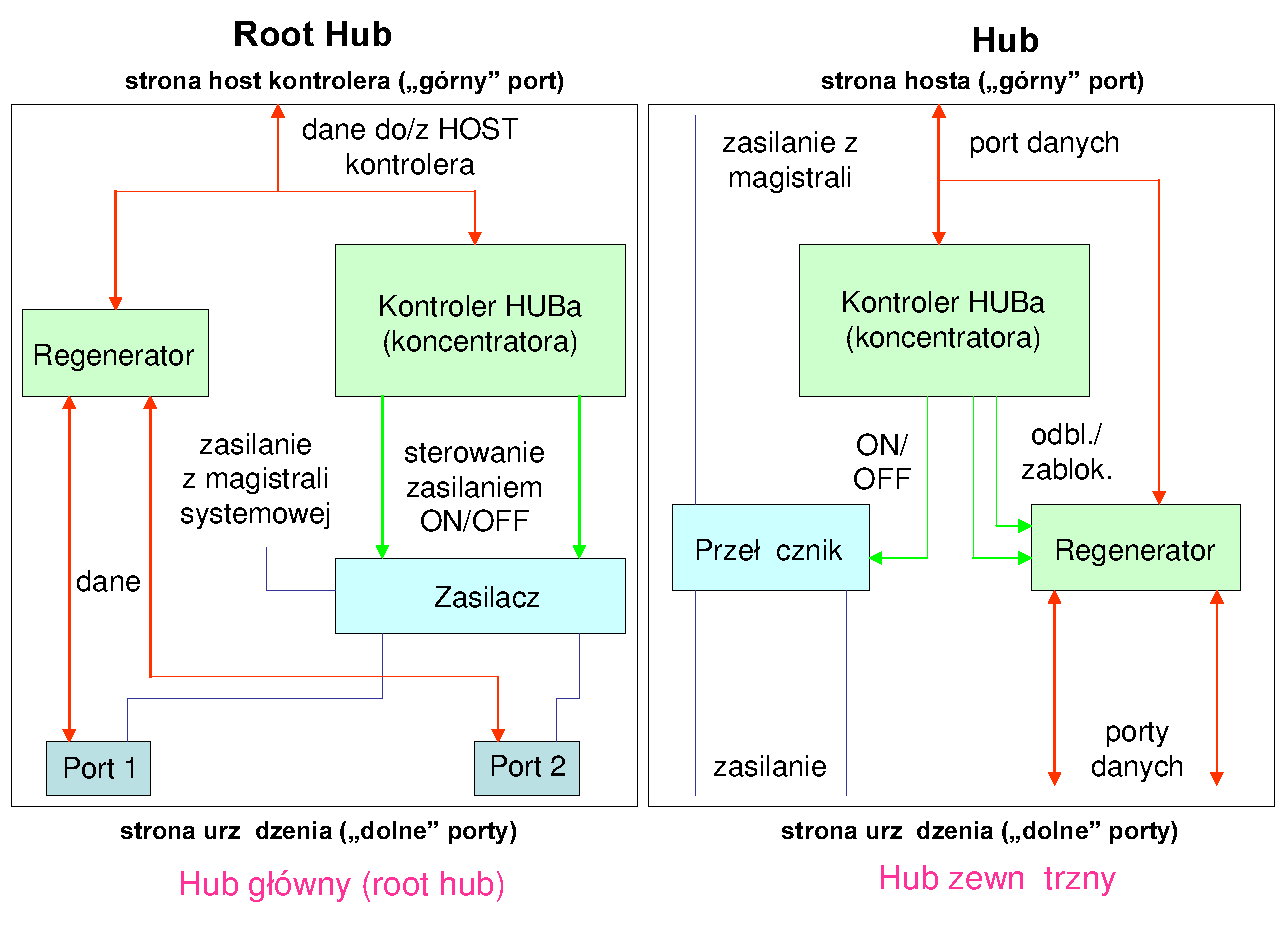
\includegraphics[width=10cm]{./wyklady/USB_17_1.pdf}
	
\subsection{Protokół komunikacyjny}
	\subsubsection{Właściwości}
	\begin{itemize}
		\item Komunikacja z urządzeniami USB za pomocą ramek o długości maksymalnej 1 ms.\\
		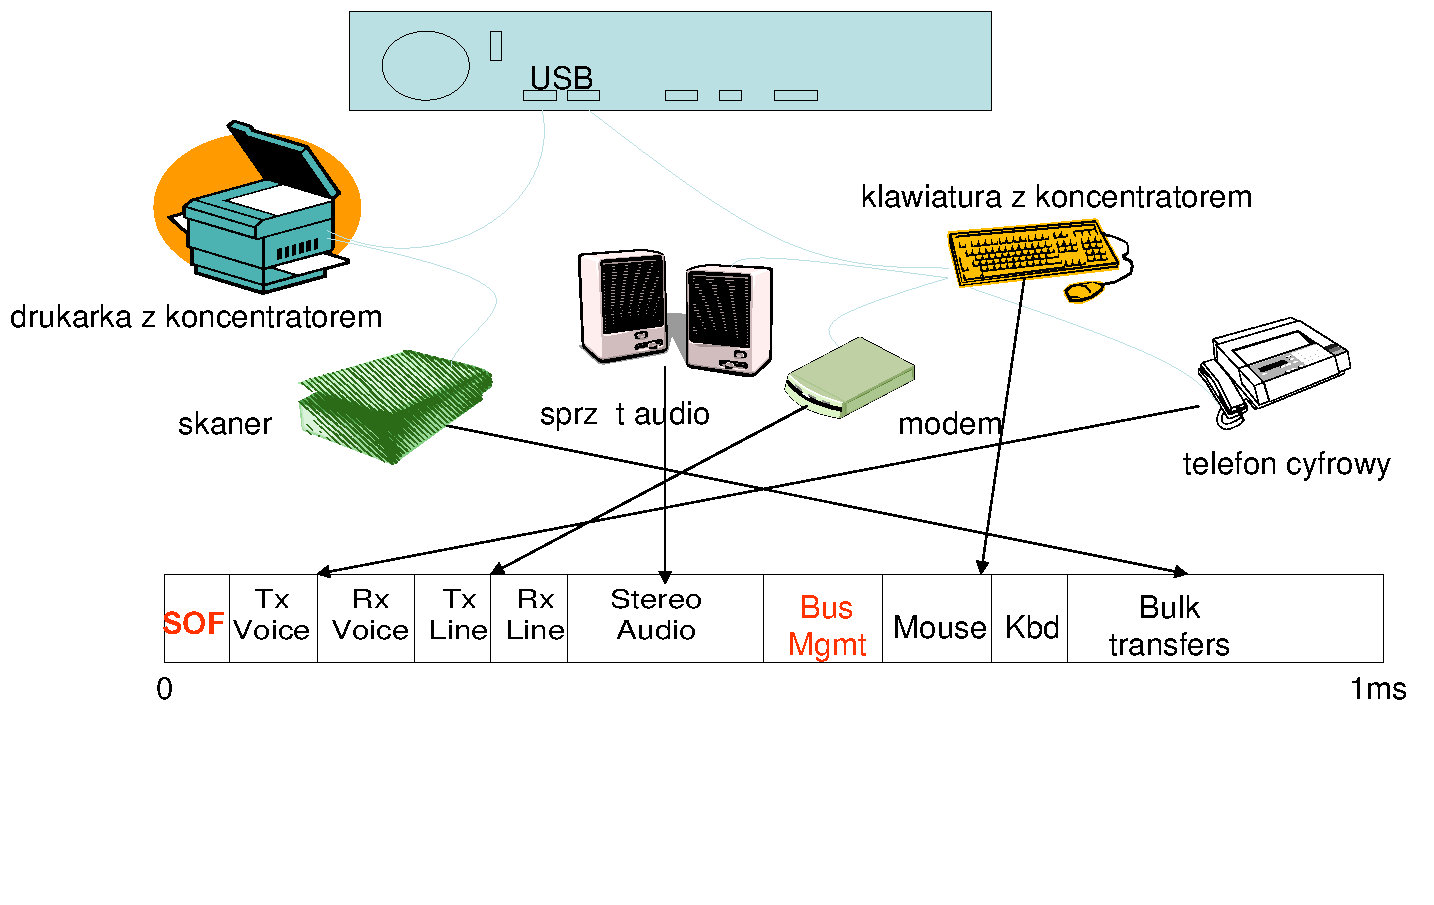
\includegraphics[width=10cm]{./wyklady/USB_18_1.pdf}
		\item Pakietowa struktura komunikatów\\
		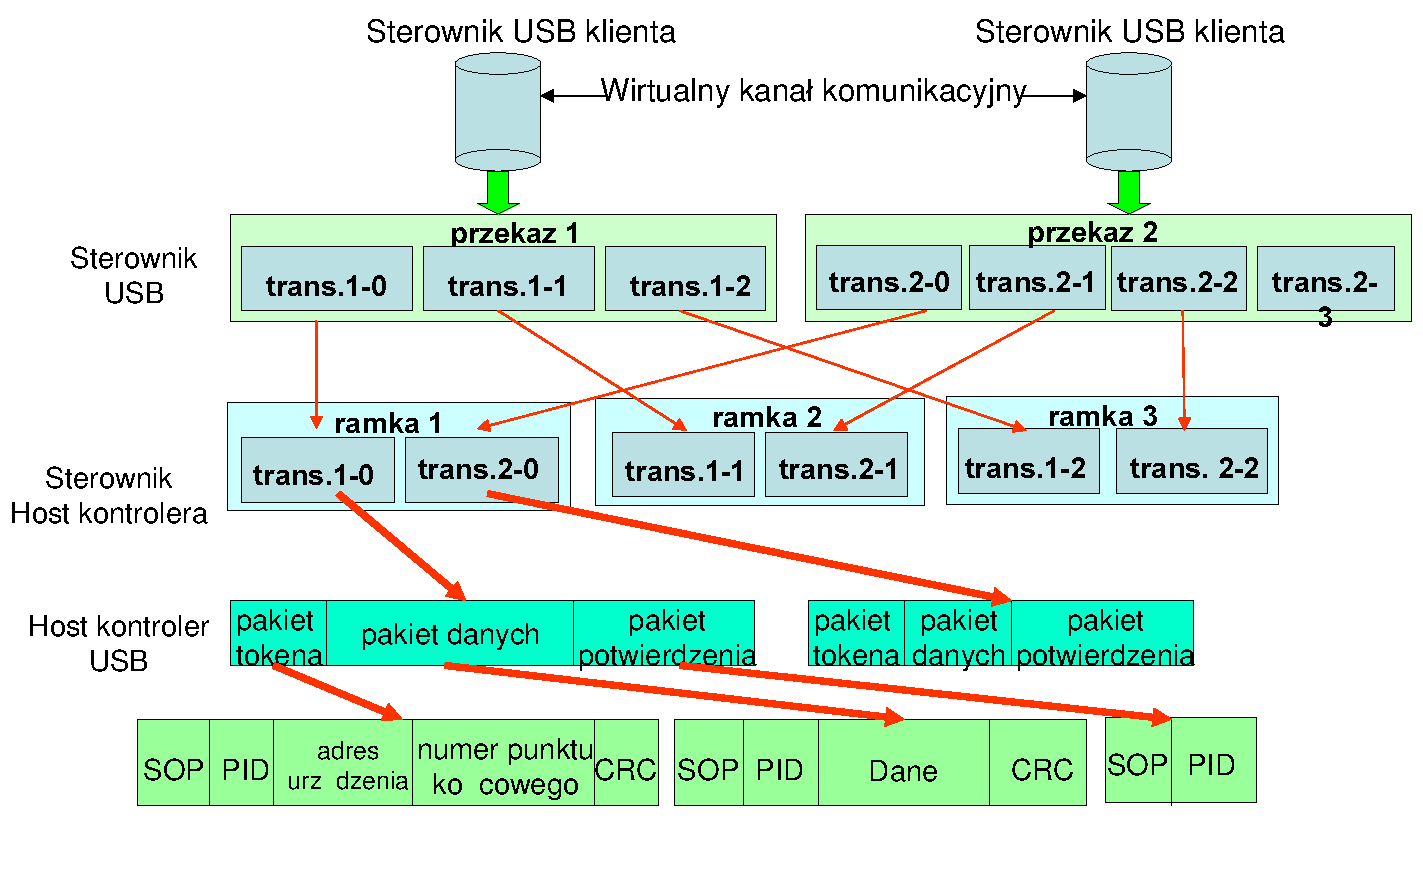
\includegraphics[width=10cm]{./wyklady/USB_19_1.pdf}\\
		Struktura bloków komunikacyjnych w USB
	\end{itemize}
	\subsubsection{Format i typy pakietów USB}
	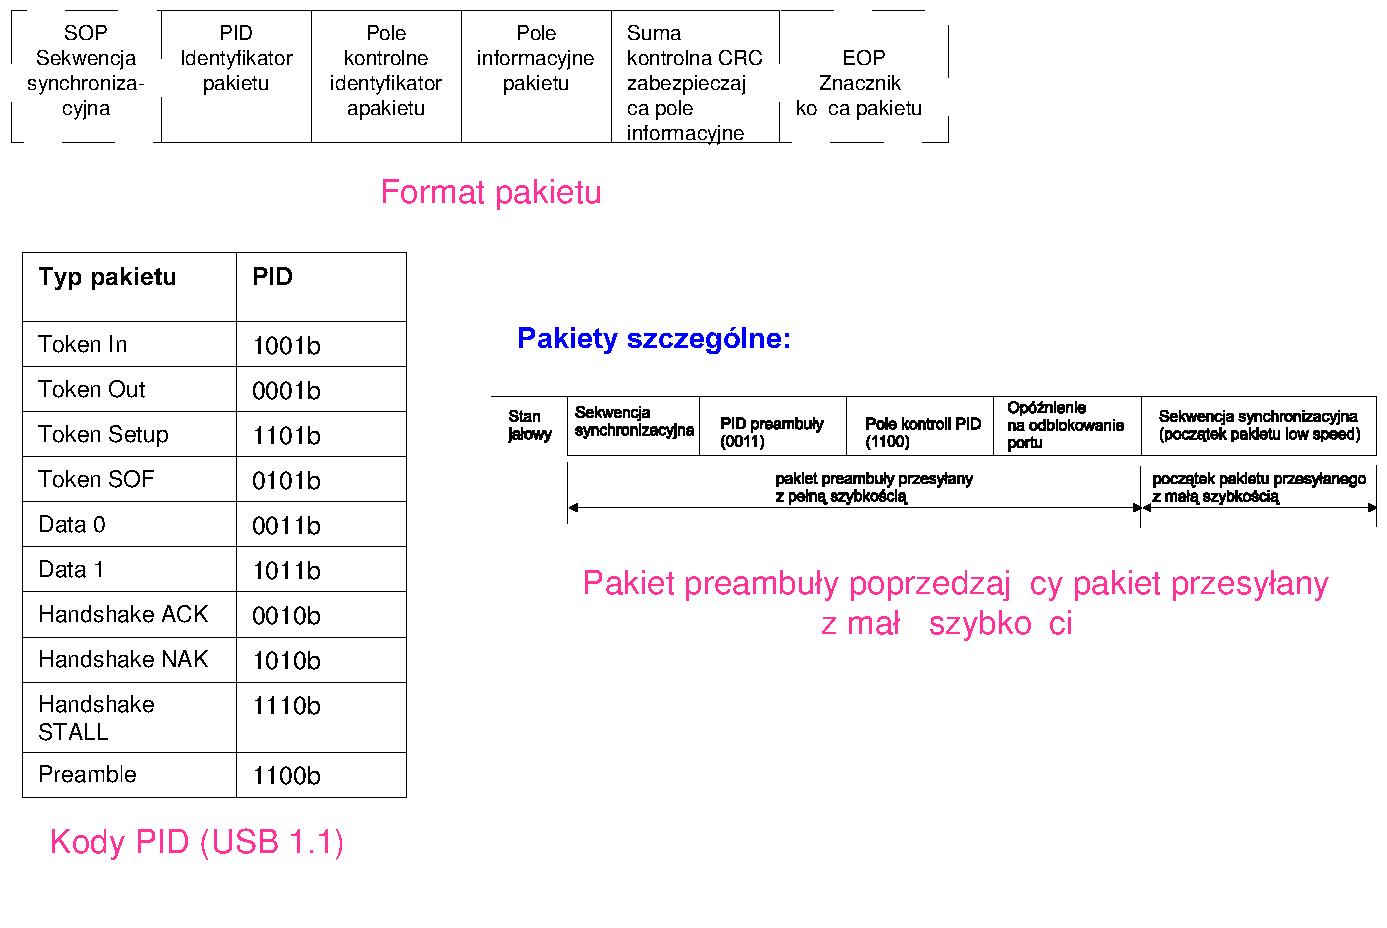
\includegraphics[width=10cm]{./wyklady/USB_20_1.pdf}
	\subsubsection{Reakcja na błędy}
	Wykrywanie błędów i kontrola transmisji\\
	\begin{itemize}
		\item Kontrola poprawności pakietów (zabezpieczenie pola PID, CRC)
		\item Reakcja na fałszywy znacznik końca pakietu (\emph{false EOP})
		\item Ograniczenie czasowe oczekiwania na odpowiedź
		\item Przełączanie kolejnych pakietów danych (mechanizm \emph{data toogle})
		\item Wykrywanie transakcji występujących po zakończeniu ramki (tzw. „paplanie” – \emph{babble})
		\item Wykrywanie braku aktywności magistrali (LOA – \emph{Loss Of Activity})
	\end{itemize}
	\subsubsection{Czas obiegu (\emph{round trip delay})}
	Ograniczenie czasowe oczekiwania na odpowiedź. Poniżej połączenie urządzenia z hostem przez 5 hubów – najgorszy przypadek.\\
	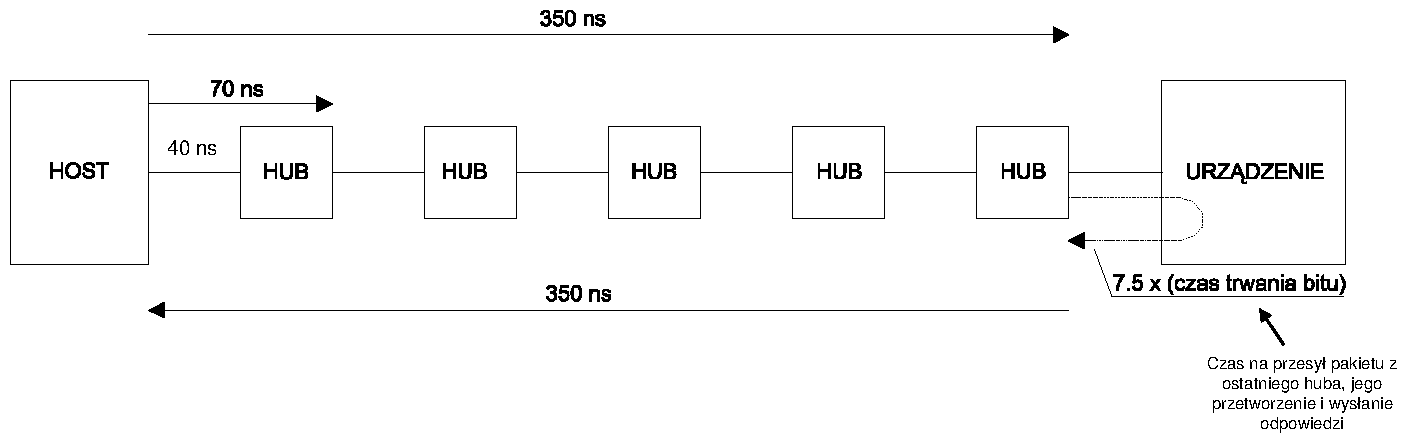
\includegraphics[width=10cm]{./wyklady/USB_23_1.pdf}
	\begin{itemize}
		\item Round trip delay: 2 x 350 ns = 700 ns
		\item Czas trwania 1 bitu full speed: 1/12 MHz = 83 ns
		\item Round trip delay w bitach dla full speed: 700 ns/83 ns = 8,5 bitu
		\item Timeout oczekiwania na odpowiedź: 7,5 bitu + 8,5 bitu = 16 bitów
	\end{itemize}
	
\subsection{Deskryptory w urządzeniach USB}
	\subsubsection{Hierarchiczna struktura deskryptorów w urządzeniu USB}
	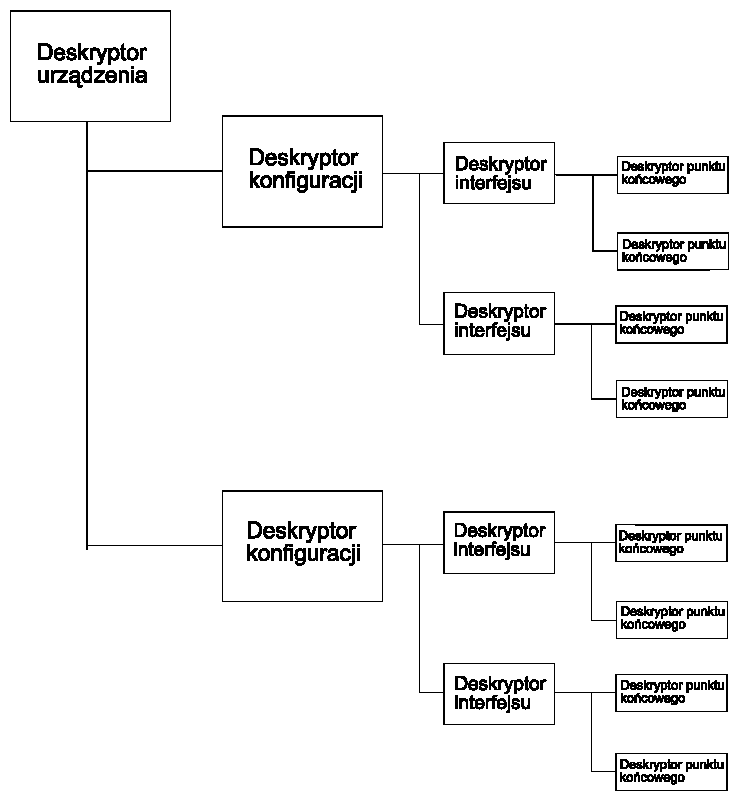
\includegraphics[width=10cm]{./wyklady/USB_24_1.pdf}
	\subsubsection{Rodzaje deskryptorów}
	\begin{itemize}
		\item Deskryptor urządzenia
		\item Deskryptor konfiguracji
		\item Deskryptor interfejsu
		\item Deskryptor punktu końcowego
		\item Deskryptor łańcuchowy
	\end{itemize}
	
\subsection{Wykrywanie i konfiguracja urządzeń}
	\subsubsection{Procedura enumeracji urządzenia}
	\begin{enumerate}
		\item Automatyczne wykrycie urządzenia
		\item Odblokowanie portu i generacja RESETU
		\item Odczyt deskryptora urządzenia
		\item Przypisanie adresu
		\item Odczyt pozostałych deskryptorów
		\item Konfiguracja urządzenia
		\item Instalacja sterownika klienta
		\item Urządzenie jest dostępne dla aplikacji
	\end{enumerate}
	
\subsection{Kontrola urządzenia – transfer kontrolny}
	\subsubsection{Etapy transferu kontrolnego}
	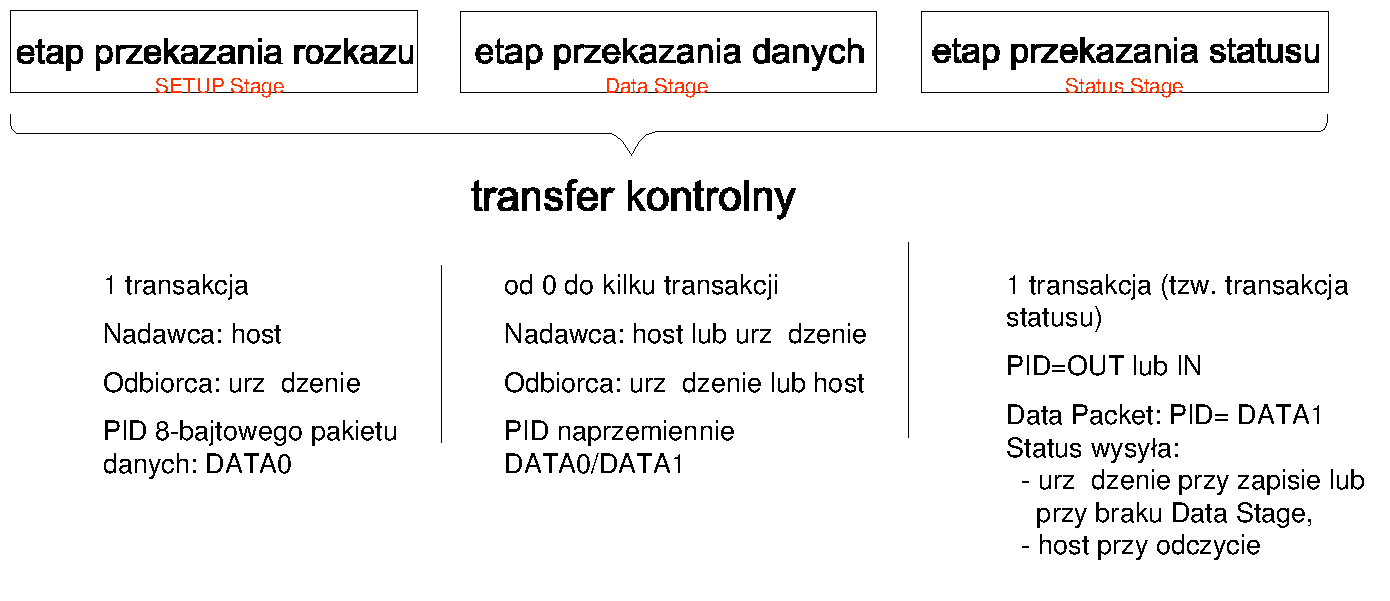
\includegraphics[width=10cm]{./wyklady/USB_31_1.pdf}
	
\subsection{Hub USB}
	\subsubsection{Co to jest?}
	Standard USB definiuje oddzielną klasę urządzeń: klasa HUB.
	\subsubsection{HUB zasilany z magistarli}
	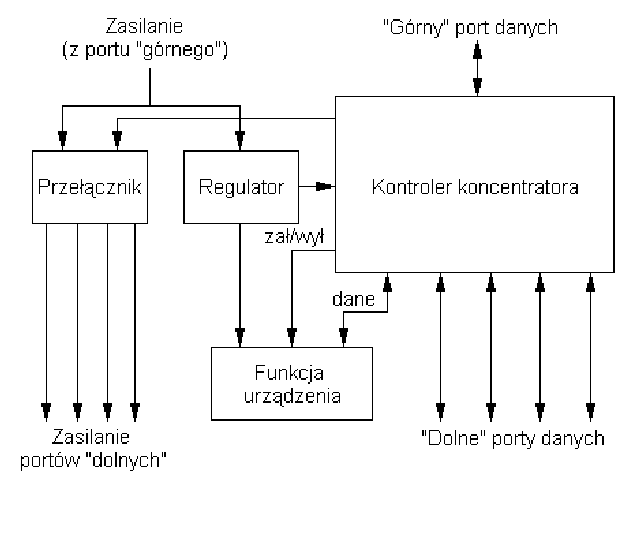
\includegraphics[width=10cm]{./wyklady/USB_34_1.pdf}
	\subsubsection{Proces konfiguracyjny huba}
	\begin{itemize}
		\item Odczyt standardowych deskryptorów urządzenia
		\item Przypisanie hubowi adresu
		\item Załączenie zasilania na porty, co jest niezbędne do detekcji podłączonych do portu urządzeń
		\item Odczyt punktu końcowego, "zmiany w hubie", w celu wykrycia urządzeń podłączonych do portów
		\item Odblokowanie portu w celu umożliwienia dostępu do urządzenia
	\end{itemize}
	\subsubsection{Punkt końcowy huba}
	\begin{itemize}
		\item \emph{Hub change point}: informuje o wystąpieniu:
		\begin{itemize}
			\item Zmiany w zasilaniu lub nadmiernym obciążeniu prądowym huba
			\item Zmiany na jednym lub kilku portach dolnych spowodowanej dołączeniem lub odłączeniem urządzenia.
		\end{itemize}
		\item Odczyt \emph{Hub change point} zwraca bajt statusowy huba
	\end{itemize}
	\subsubsection{Działanie}
	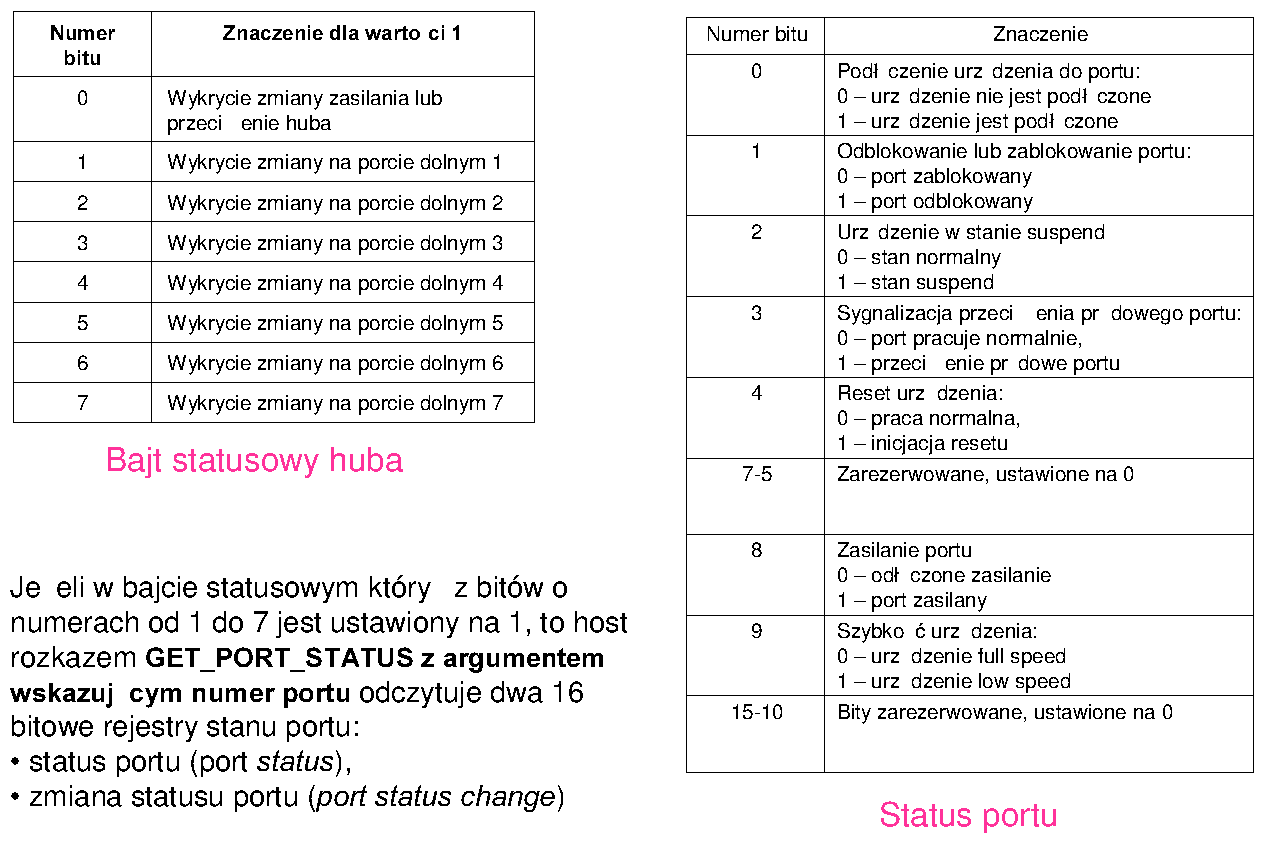
\includegraphics[width=8cm]{./wyklady/USB_35_1.pdf}
	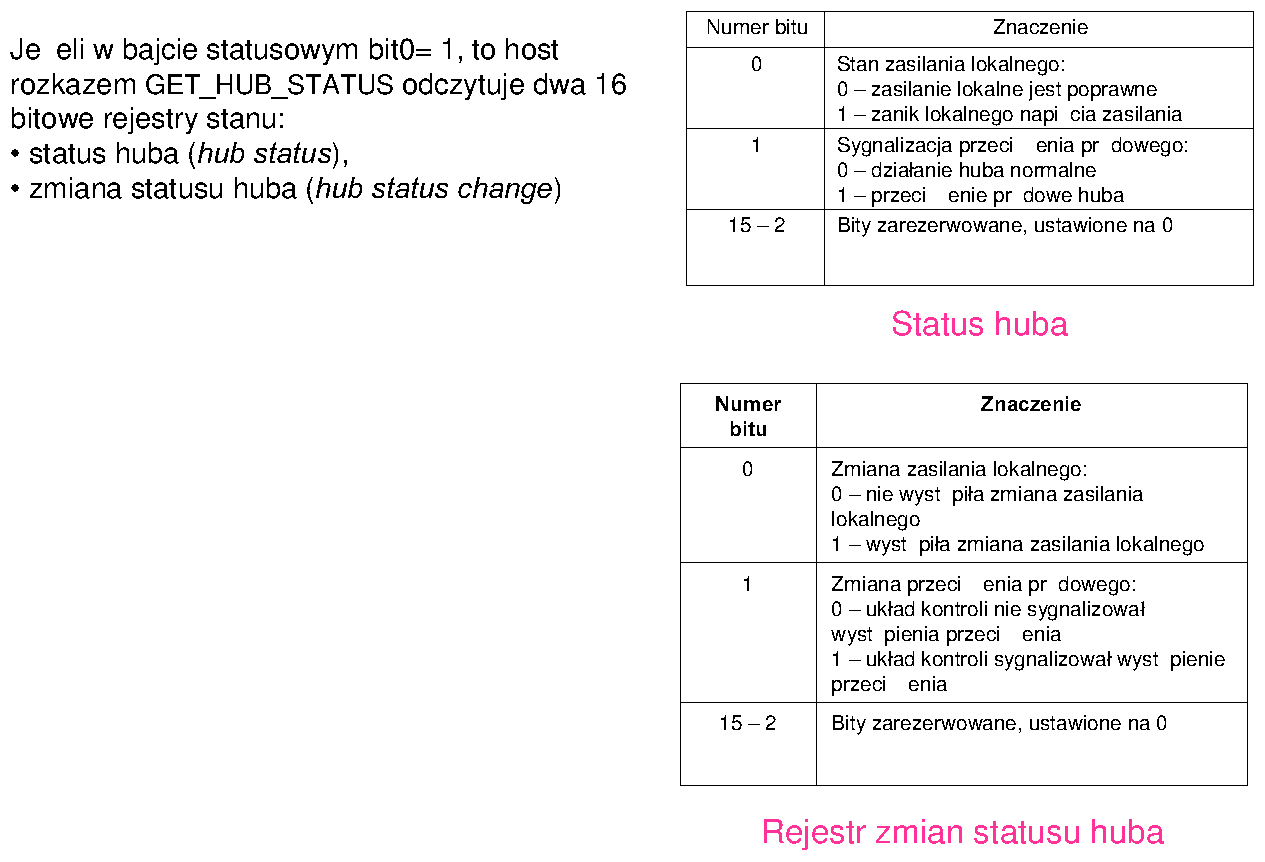
\includegraphics[width=8cm]{./wyklady/USB_36_1.pdf}
	
\subsection{Zasilanie urządzeń w systemie USB}
	\subsubsection{Rodzaje zasilania urządzeń USB}
	\begin{itemize}
		\item Urządzenie zasilane z magistrali
		\item Urządzenie zasilane z własnego źródła
		\item Urządzenie zasilane częściowo z magistrali i własnego źródła
	\end{itemize}
	\subsubsection{Zasilanie hubów i pozostałych urządzeń}
		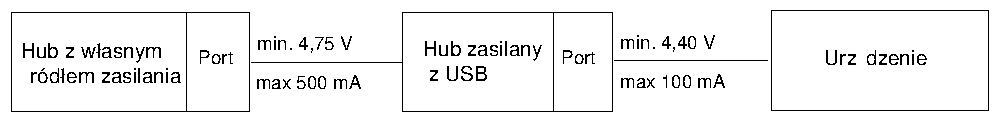
\includegraphics[width=11cm]{./wyklady/USB_38_1.pdf}\\
		Dopuszczalne spadki napięcia zasilania.
	\subsubsection{Urządzenie zasilane z magistrali}
		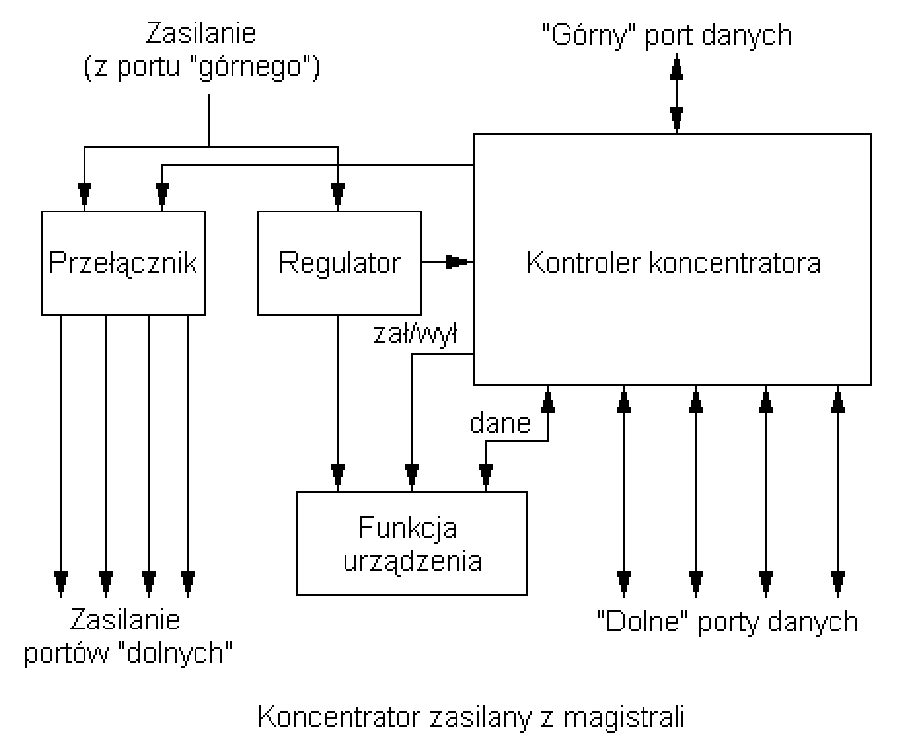
\includegraphics[width=7cm]{./wyklady/USB_39_1.pdf}
	\subsubsection{Zarządzanie zasilaniem}
	\begin{itemize}
		\item Zawieszenie pracy systemu – \emph{SUSPEND}
		\begin{itemize}
			\item \textbf{Globalne} - rozkaz SetPortFeature (PORT\_SUSPEND) adresowany do huba głównego
			\item \textbf{Częściowe} - rozkaz SetPortFeature (PORT\_SUSPEND) adresowany do huba zewnętrznego, w którym wybrany port ma zostać zawieszony.
			\item Zawieszone porty nie propaguj ruchu „w dół” oraz nie przekazuj „w gór ” żadnych sygnałów od urządzeń do nich podłączonych.
			\item Urządzenia w stanie zawieszenia zachowuj swój stan, co umożliwia wznowienie ich pracy bez ponownej konfiguracji.
			\item Hub w stanie zawieszenia dodatkowo blokuje wszystkie nadajniki, zatrzymuje wewnętrzne zegary i zachowuje stan wszystkich portów dolnych.
		\end{itemize}
		\item Wznowienie pracy systemu - \emph{RESUME} - po zawieszeniu
		\begin{itemize}
			\item Globalne
			\item Wake-up
			\item Wznowienie pracy urządzenia można nastąpić
			\begin{itemize}
				\item Z inicjatywy kontrolera, jako wznowienie po zawieszeniu globalnym lub częściowym\\
				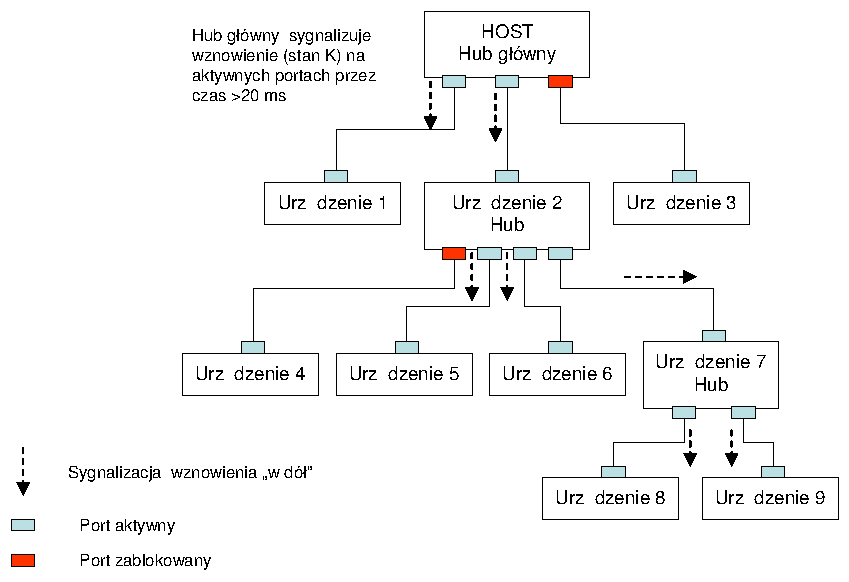
\includegraphics[width=7cm]{./wyklady/USB_43_1.pdf}
				\item Z inicjatywy urządzenia, po wystąpieniu zdarzenia wymagającego obsługi („budzenie” - \emph{Wakeup})\\
				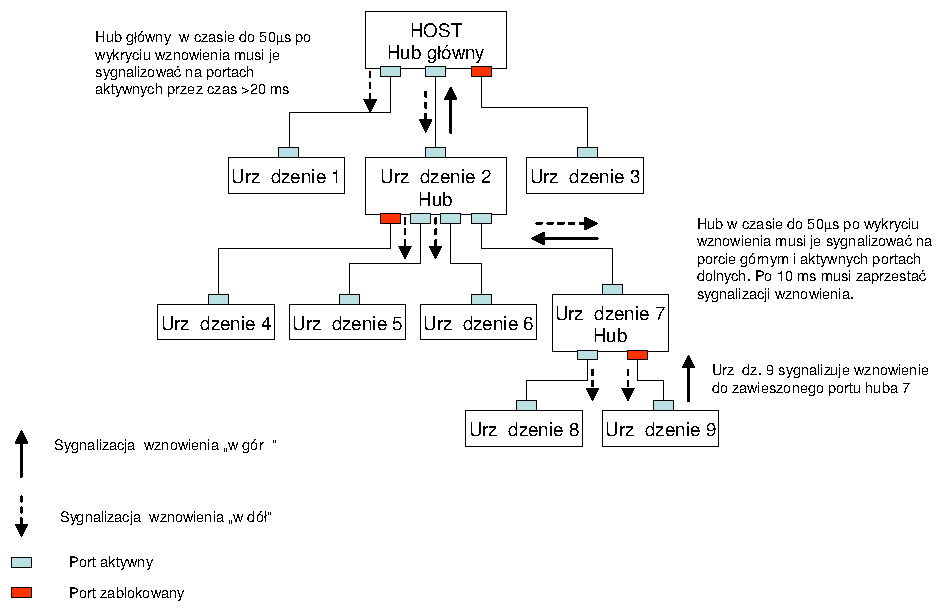
\includegraphics[width=7cm]{./wyklady/USB_44_1.pdf}
			\end{itemize}
			\item Wznowienie po zawieszeniu globalnym - rozpoczyna hub główny wykonując rozkaz wznowienia pracy systemu
			\item Wznowienie po częściowym zawieszeniu - może wykonać:
			\begin{itemize}
				\item Host rozkazem \emph{ClearPortFeature} (PORT SUSPEND) adresowanym do huba w którym znajduje się zawieszony port
				\item Urządzenie podłączone do zawieszonego portu poprzez \emph{Wakeup}
			\end{itemize}
		\end{itemize}
		\item Urządzenie pełnej szybkości (\emph{full speed}) automatycznie przechodzi do stanu \emph{SUSPEND} po wykryciu braku aktywności magistrali przez 3 $ms$.
		\item Urządzenie w stanie zawieszenie pobiera prąd $< 500 [\mu A]$
	\end{itemize}
\subsection{Rozwiązania host kontrolerów}
	\subsubsection{Co to jest?}
	Opracowano dwa rozwiązania host kontrolera:
	\begin{itemize}
		\item Uniwersalny host kontroler - \emph{Universal Host Controler} (Intel)
		\item Otwarty host kontroler – \emph{Open Host Controler} (Compaq, Microsoft, National Semiconductor)
	\end{itemize}
	\subsubsection{Uniwersalny host kontroler (UHC)}
	\textbf{Zasada działania kontrolera UHC}\\
	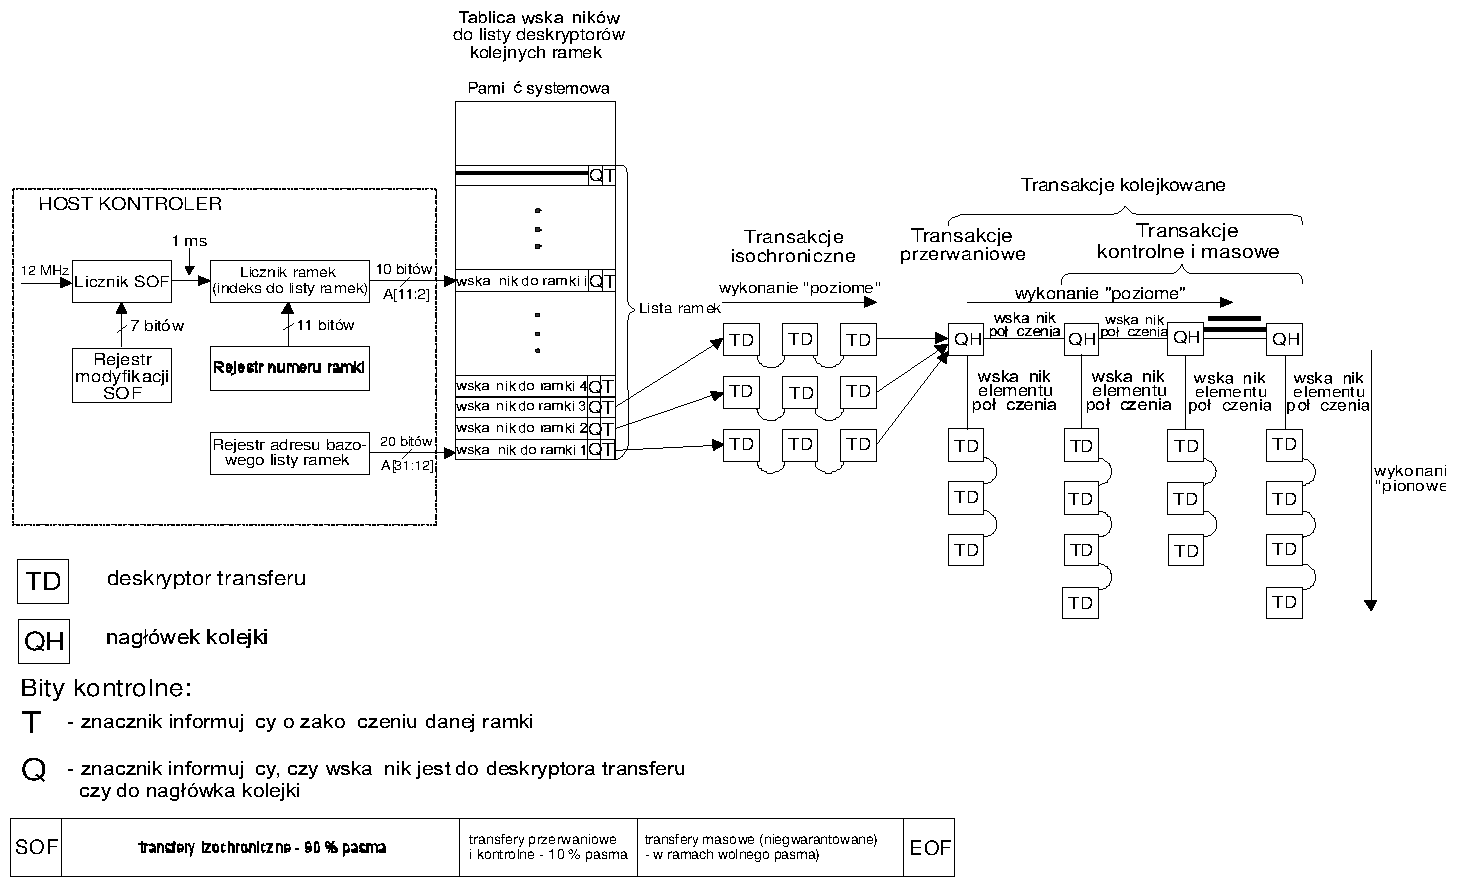
\includegraphics[width=7cm]{./wyklady/USB_46_1.pdf}\\\\
	\textbf{Ogólna postać deskryptora transferu (TD)}\\
	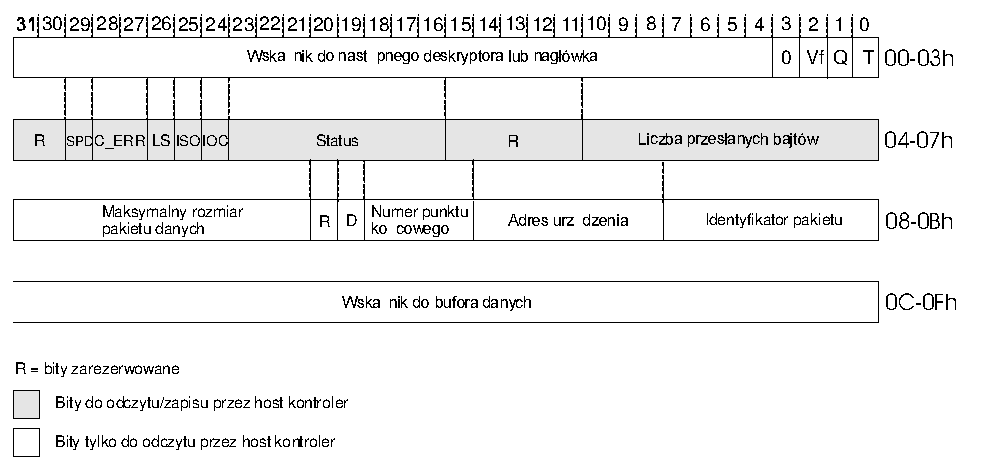
\includegraphics[width=7cm]{./wyklady/USB_47_1.pdf}\\\\
	\textbf{Ogólna postać nagłówka kolejki (QH)}\\
	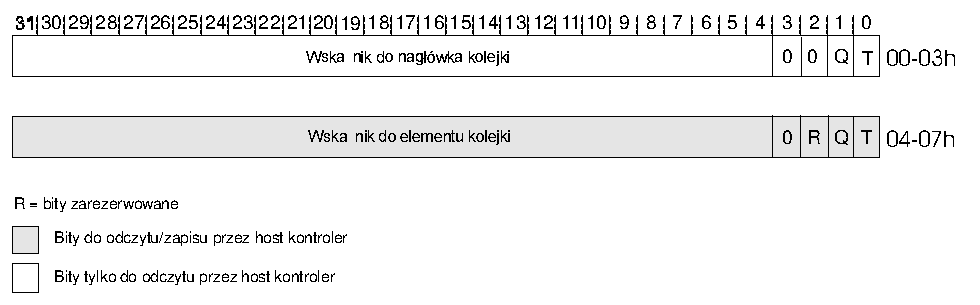
\includegraphics[width=7cm]{./wyklady/USB_48_1.pdf}
	\subsubsection{Otwarty host kontroler (OHC)}
	\textbf{Zasada działania kontrolera OHC}\\
	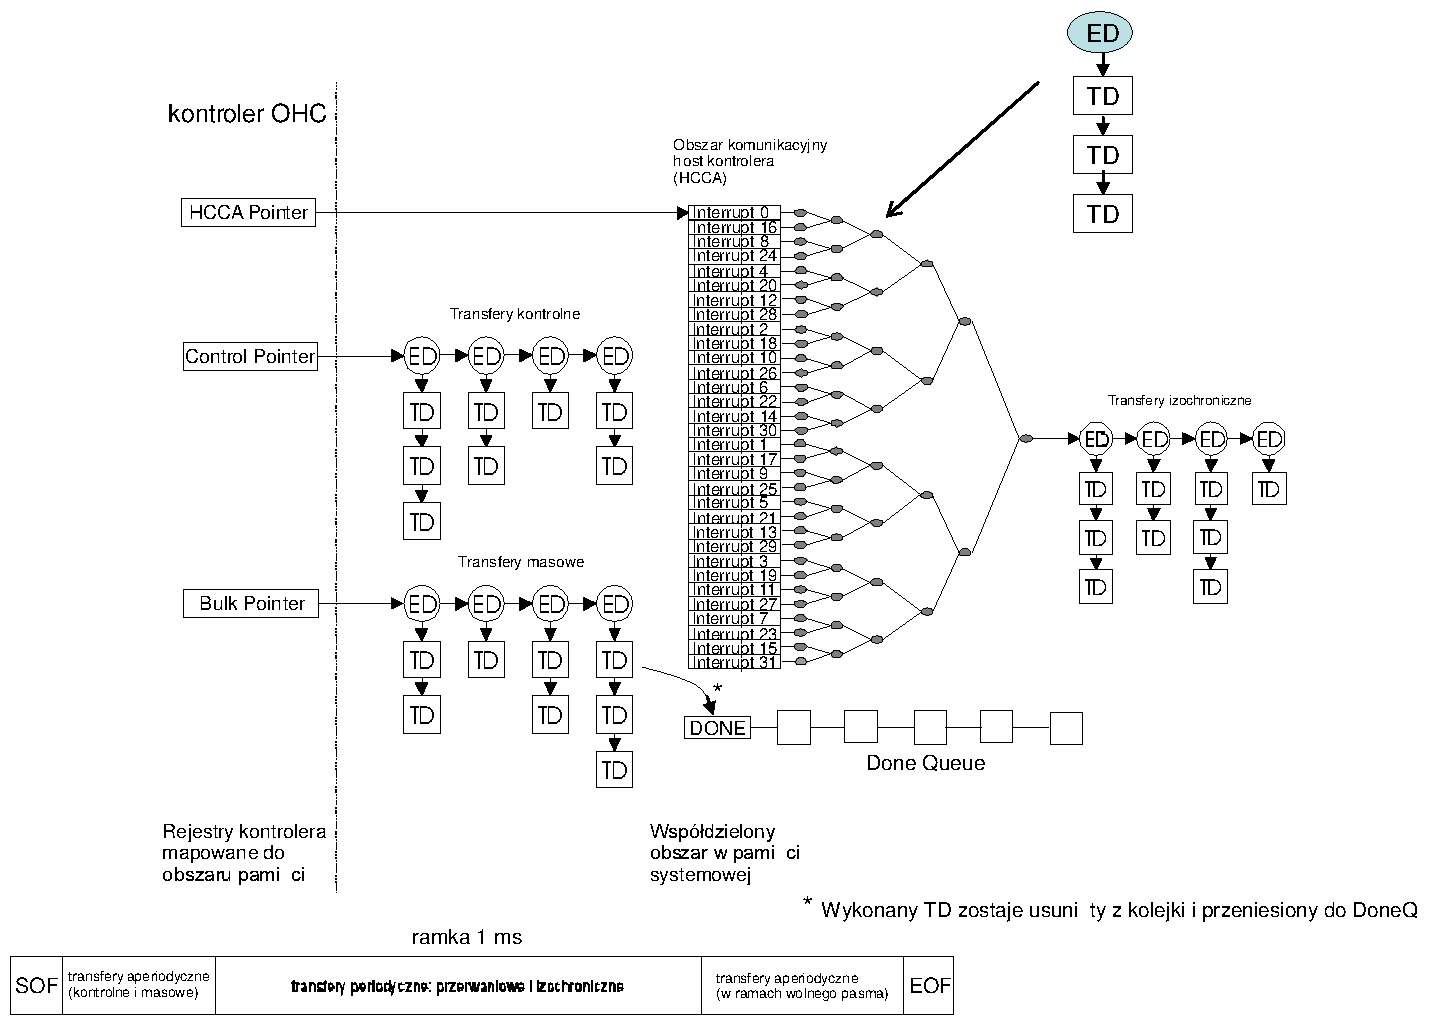
\includegraphics[width=7cm]{./wyklady/USB_49_1.pdf}\\\\
	\textbf{Format deskryptora punktu końcowego (ED)}\\
	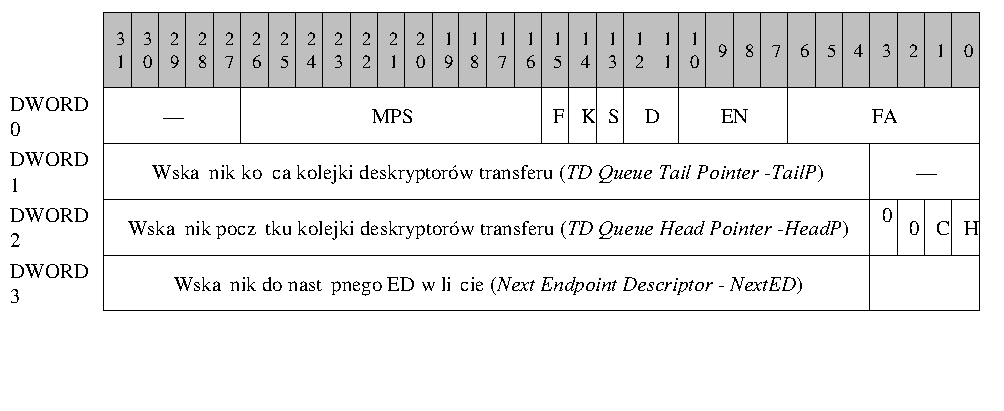
\includegraphics[width=7cm]{./wyklady/USB_50_1.pdf}\\\\
	\textbf{Ogólna postać deskryptora transferu (TD)}\\
	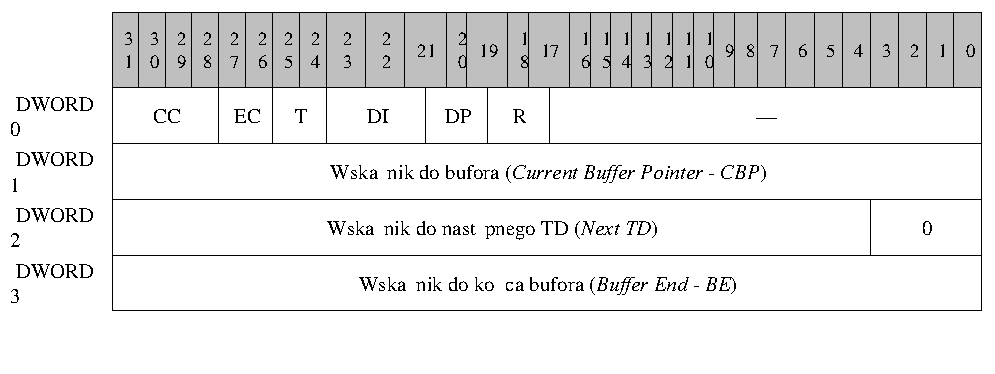
\includegraphics[width=7cm]{./wyklady/USB_51_1.pdf}
	
\subsection{USB 2.0 - rozszerzenie standardu}
	\subsubsection{Ważniejsze elementy wprowadzone w USB 2.0}
	\begin{itemize}
		\item Wysoka szybkość transmisji (high speed) - 480 Mb/s
		\item Protokół PING-NYET
		\item Transakcja SPLIT
		\item Komunikacja z szerokopasmowym punktem izochronicznym
		\item Nowe typy pakietów
	\end{itemize}
	\subsubsection{Wysoka szybkość transmisji}
	Podział ramki na 8 mikroramek wysokiej szybkości\\
	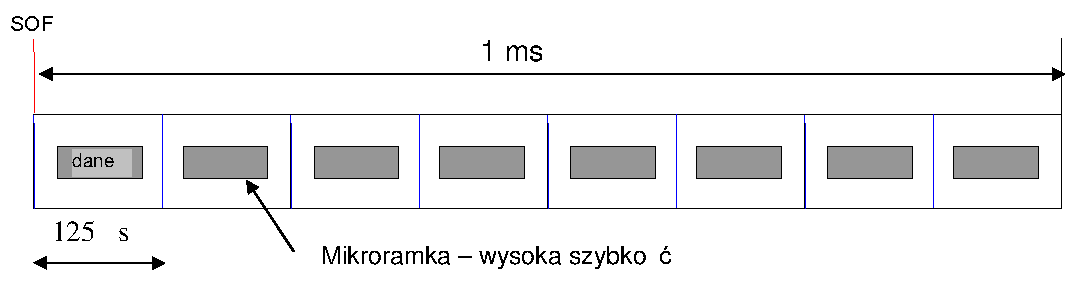
\includegraphics[width=7cm]{./wyklady/USB_53_1.pdf}
	\begin{itemize}
		\item Mikroramka trwa 125 $\mu s$
		\item Na 1 ramkę przypada 8 mikroramek
		\item Wysoka szybkość transmisji - w mikroramce wynosi 480 Mhz.
	\end{itemize}
	\subsubsection{Protokół PING-NYET}
	Potwierdzenie NYET (\emph{NOT YET}) dla urządzeń \emph{high speed}.\\
	\textbf{Problem:} przy zapisie do urządzenia, jeżeli nie jest ono „gotowe na dane” potwierdzenie negatywne przychodzi dopiero po pakiecie danych – strata czasu.\\
	\textbf{Rozwiązanie}:\\
	TOKEN PING – zapytanie urządzenia, czy jest gotowe do przyjścia danych.\\
	Możliwe odpowiedzi i reakcja hosta:
	\begin{itemize}
		\item ACK – wykonanie transakcji OUT
		\item NYRT – host kontynuuje wysyłanie zapyta PING
	\end{itemize}
	\textbf{Korzyści}: lepsze wykorzystanie magistrali (PING jest krótki).
	\subsubsection{Transakcja SPLIT}
	\textbf{Problem:} Host i hub wysokiej szybkości komunikują się z urządzeniem małej lub pełnej szybkości. Szybkie przesyłanie danych pomiędzy hostem i hubem oraz wolne pomiędzy hubem i urządzeniem – konieczność buforowania danych w hubie.\\
	\textbf{Rozwiązanie}:\\
	Transakcja dzielona, złożona z dwóch części:
	\begin{itemize}
		\item SSPLIT (\emph{Start Split} - rozpoczęcie transakcji dzielonej)
		\item CSPLIT (\emph{Complete Split} – zakończenie transakcji dzielonej).
	\end{itemize}
	\subsubsection{Komunikacja z szerokopasmowym punktem izochronicznym}
	Komunikacja z „normalnym” izochronicznym punktem końcowym zakłada jedną transakcję na ramę lub mikroramkę.\\
	W przypadku punktów szerokopasmowych, obsługiwanych tylko przez kanały \emph{high speed}, istnieje możliwość przekazania w jednej mikroramce większej ilości danych wykonując bezpośrednio po sobie od jednej do trzech transakcji.\\
	Dane w takiej sekwencji transakcji muszą być oznaczone, przy czym nie wystarczą już „znaczniki” Data 0 i Data 1, dlatego wprowadzono dwa kolejne typy pakietów danych: \textbf{Data 2} i \textbf{MData}.\\
	Pakiet \textbf{Data 2} wykorzystywany jest przy odczycie danych z urządzenia, natomiast \textbf{MData} i \textbf{Data 2} przy zapisie do urządzenia.\\
	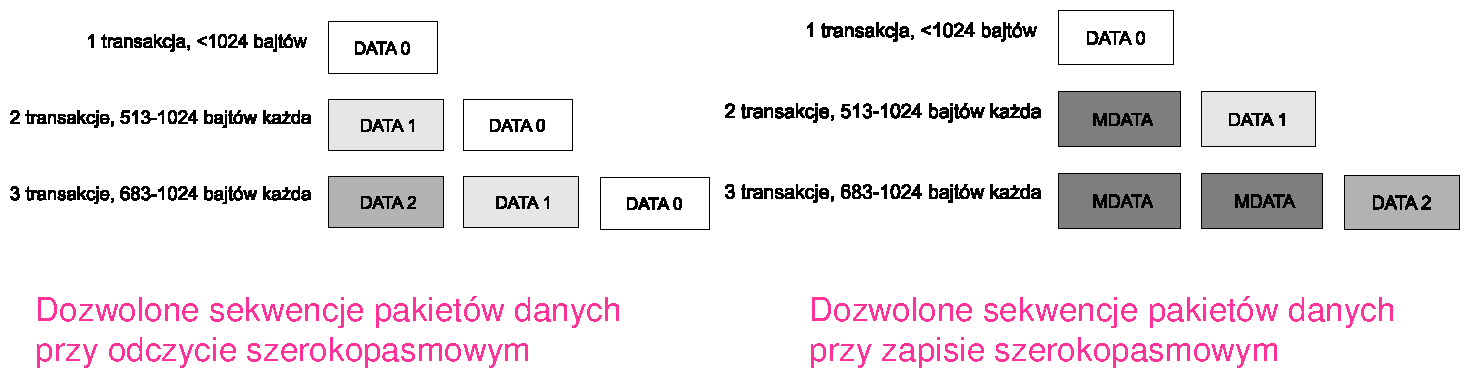
\includegraphics[width=15cm]{./wyklady/USB_56_1.pdf}
	\subsubsection{Specjalne pakiety TOKEN wprowadzone w USB 2.0}
	Kody pakietów specjalnych zgodnie z USB 2.0\\
	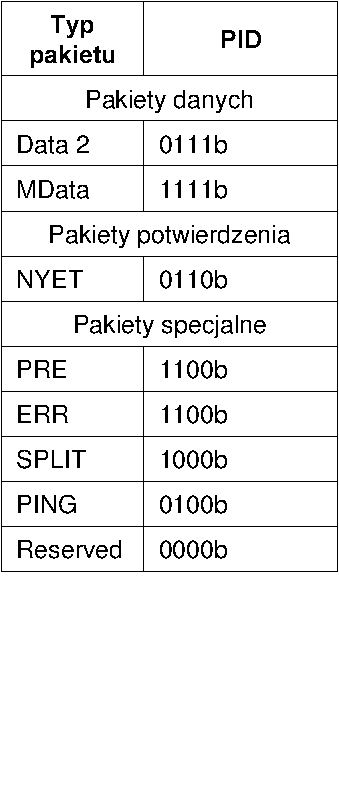
\includegraphics[width=3cm]{./wyklady/USB_57_1.pdf}